\subsection{The Challenges: Foregrounds, systematics}
\label{sec:foregrounds}
\vspace{-0.05in}
\comred{3 pages. Discuss the challenge of Foregrounds and Systematics. }
%A satellite mission provides a unique opportunity to target both the inflationary B-mode polarization that originates from the epoch of recombination and peaks around $\ell=80$ and the contribution that peaks on significantly larger scales $\ell\lesssim 12$. To measure the contribution from reionization will require an unprecedented understanding of foregrounds and systematic effects. This is illustrated in the left panel of Figure~\ref{fig:Qrp001}, which shows the contribution from reionization to the Stokes $Q$-parameter for $r=0.001$. The amplitude of the signal is approximately $10$ nK

The search for primordial B-modes is one of the main science objectives of any future CMB mission. A satellite mission is the most sensitive probe of this signal from the early universe because it can access the full sky and the choice of frequencies is not limited by the atmosphere. 

By the time of launch of a probe class mission substantial progress will already have been made. In the case of a detection at the time of launch, the probe mission should be able to convincingly detect the expected reionization signal. In the absence of a signal it should significantly improve the upper limits beyond $\sigma(r)=0.001$. 

The contribution from reionization to the Stokes $Q$-parameter for a tensor-to-scalar ratio $r=0.001$ is shown in the left panel of Figure~\ref{fig:Qrp001}. The amplitude of the signal is approximately $10$ nK so that any experiment attempting to measure such a signal must control foregrounds and systematics on large angular scales at an unprecedented level of a few nK. 

\begin{figure}[h]
\begin{center}
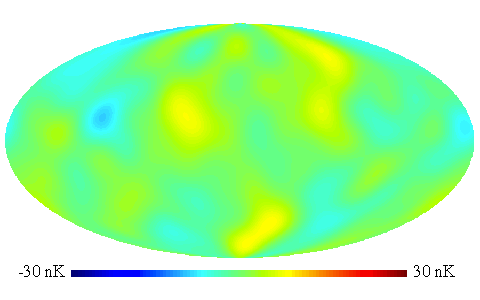
\includegraphics[width=3.2in]{Figures/P15_2_12_rp001.pdf}
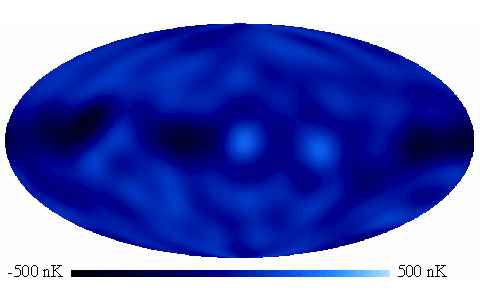
\includegraphics[width=3.2in]{Figures/P353_N_2_12.pdf}
\end{center}
\caption{{\it Left panel:} Contribution to the Stokes $Q$ parameter from inflationary B-modes for $\ell<12$ for $r=0.001$. {\it Right panel:} Noise in the $Planck$ 353 GHz map of the Stokes $Q$ parameter for $\ell<12$ rescaled to 150 GHz assuming the spectral properties of dust.}
\label{fig:Qrp001}
\end{figure}
\subsubsection{Foregrounds}
Data from the $Planck$ satellite has significantly improved our understanding of foregrounds in both intensity and polarization. 
%In intensity, $Planck$, for example, showed the unexpected relevance of Carbon-Monoxide lines at moderate latitudes as well as the existence of an anomalous emission from dust at low frequencies. 
In polarization, the sky is dominated by the expected sources, synchrotron and dust, and $Planck$ has provided us with much improved measurements of their amplitude and spectral dependence. The observed spectral dependence is shown in the left panel of Figure~\ref{fig:frequency} for different sky fractions. One of the most important lessons is that foregrounds are larger than putative primordial B-mode signal everywhere. 

This is particularly severe on the scales relevant for the search of primordial B-modes as can be seen in the right panel of Figure~\ref{fig:frequency}, which shows the power spectrum of foregrounds over $75\%$ of the sky for frequencies between $70$ and $200$ GHz together with the lensing and inflationary contribution for different values of the tensor-to-scalar ratio.

Perfect knowledge of the foreground components would allow to remove them, but the sensitivity of Planck limits our ability. The right panel in Figure~\ref{fig:Qrp001} shows the noise in the $Planck$ 353 GHz map of the Stokes $Q$-parameter rescaled to 150 GHz assuming the same spectral dependence as for dust and on the angular scales relevant for the measurement of the inflationary $B$-modes. The noise is more than an order of magnitude larger than the inflationary contribution for $r=0.001$, clearly indicating the necessity to measure foregrounds with a potential future space mission. A probe class mission likely is the only way to map foregrounds at a level required to measure primordial gravitational waves for $r<0.001$. 

While the search for primordial B-modes leads to the strictest constraints on foreground residuals, exquisit control of foregrounds is also necessary for other science objectives. A satellite mission is likely also the only reliable way to measure the optical depth at a level necessary to break the degeneracy with the neutrino mass. Furthermore, a cosmic variance limited measurement of E-mode polarization on large scales possible with a probe mission would contain valuable information about the star formation history. 

Similarly, a clear objective of the spectral science is to have a robust, foreground-marginalized expectation of detecting the $\mu$-distortion generated by the dissipation of small-scale acoustic modes in $\Lambda$CDM. While an instrument like PIXIE just falls short of this objective, it seems within reach of a probe mission.

\begin{figure}[h]
\begin{center}
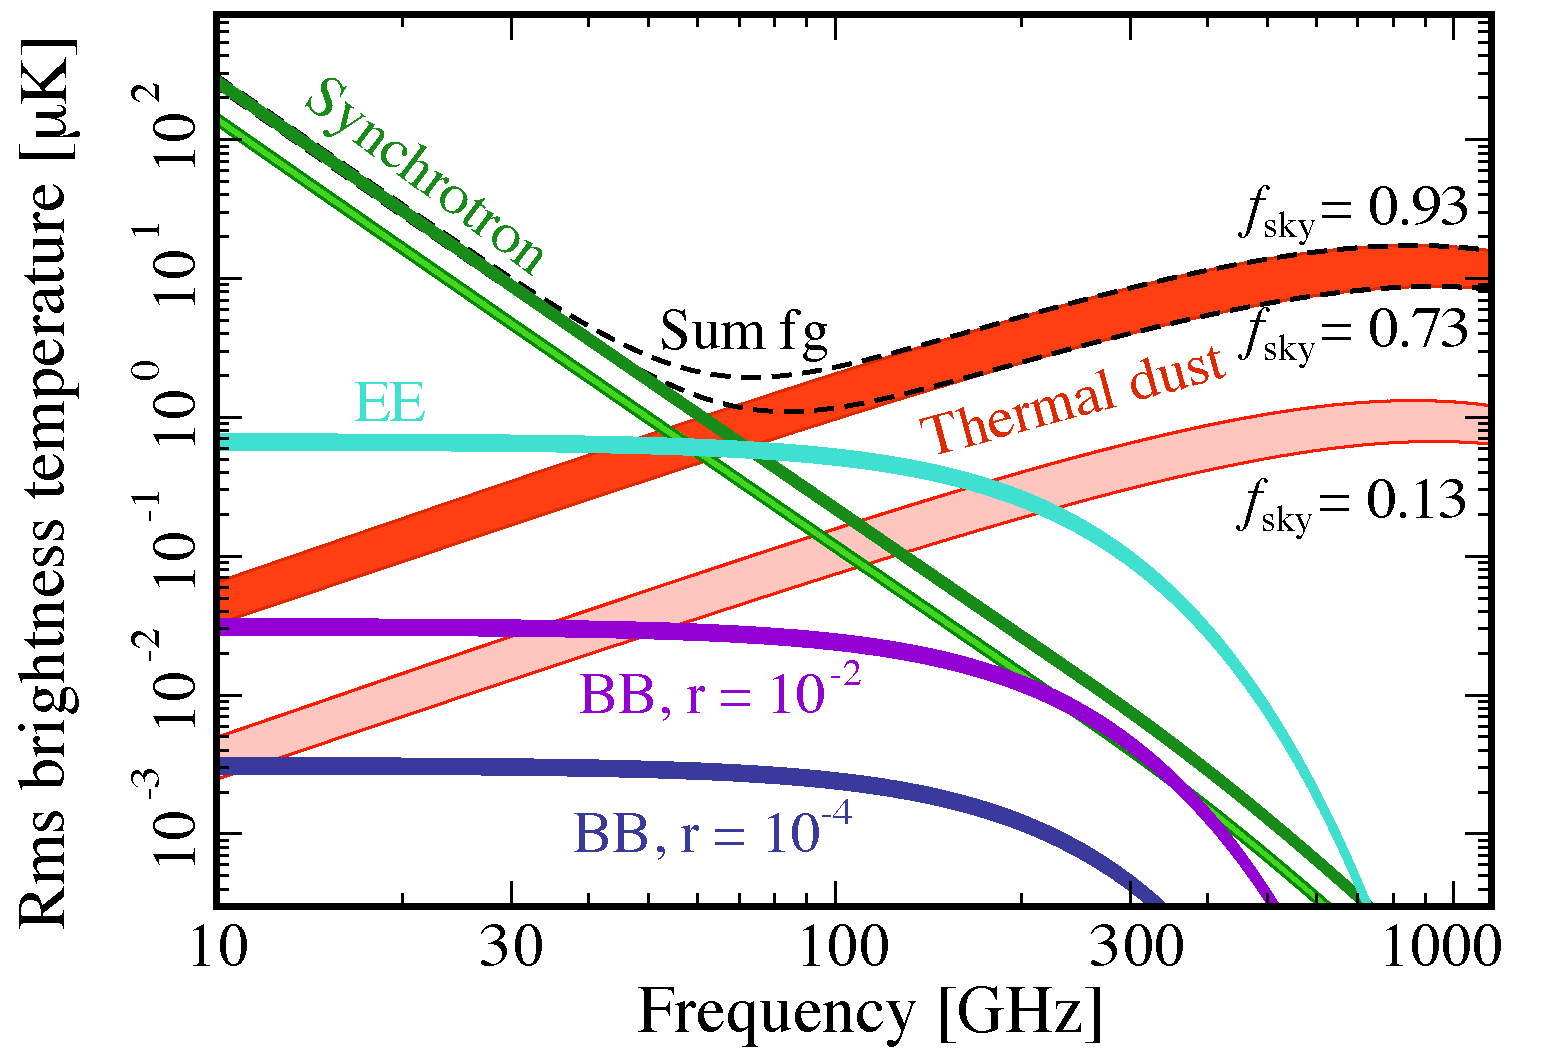
\includegraphics[width=3.26in]{Figures/overview_pol_v4_fsky_noplanck.pdf}\hskip .2cm
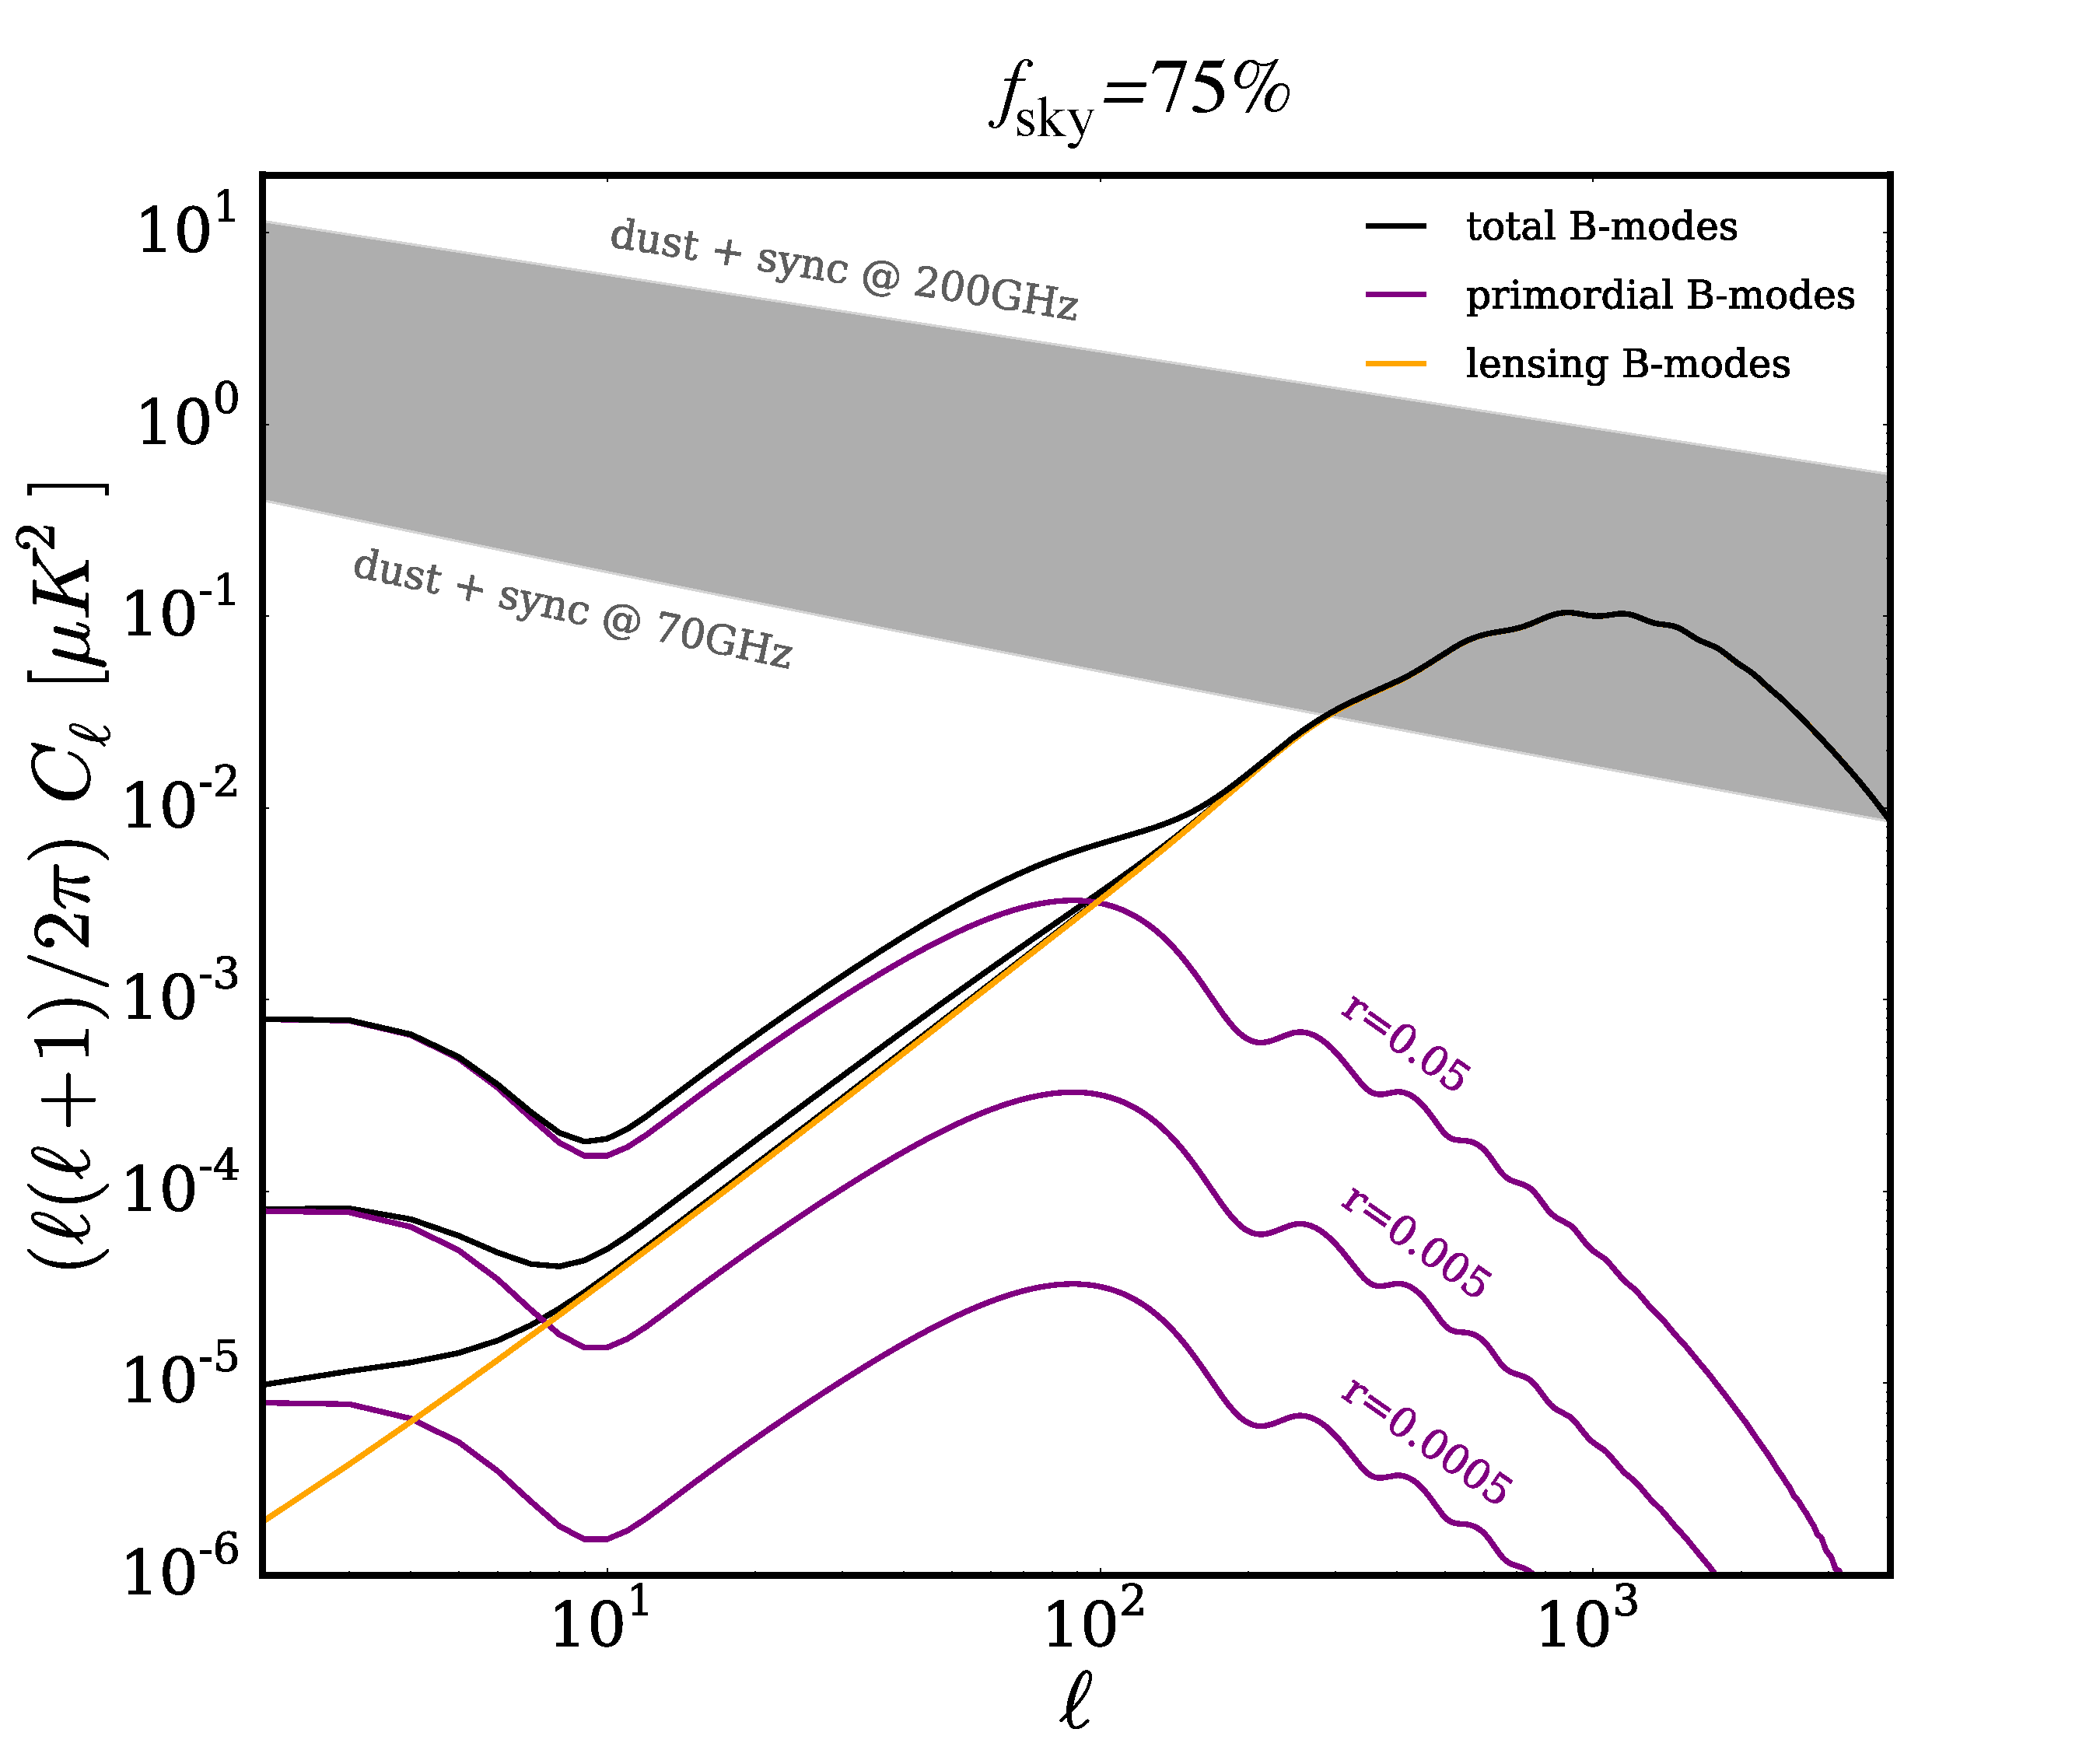
\includegraphics[width=3.12in]{Figures/clbb_freq.pdf}
\end{center}
\caption{{\it Left panel:} Brightness temperature as function of frequency for the CMB as well as synchrotron emission (green) and dust emission (red). The darker bands show the brightness temperature for sky fractions between $73\%$ and $93\%$, the lighter bands show the brightness temperature for the cleanest $13\%$ with the width indicating the uncertainty. {\it Right panel:} Angular power spectrum for B-mode polarization of the CMB for $r=0.0005$, $r=0.005$, and $r=0.05$ as well as for foreground emission between 70 and 200 GHz.}
\label{fig:frequency}
\end{figure}


One of the key ingredients in the design of a CMB experiment is the frequency coverage required to achieve the science goals. Consequently, optimizing frequency coverage in light of the new information from $Planck$ and its limitations will be one of key task of the study proposed here.   

To achieve these goals we plan to investigate the effect on the measurements of r and \tau of the presence of foregrounds residuals in the CMB maps (after foreground separation and/or cleaning) including, for example, the properties of the polarized thermal dust emission, specifically the potential spatial variation of its spectral index, hinted at by the observed decorrelation of the dust between 217 GHz and 353GHz Planck channels (\ref{Planck2015-X;Planck2015-L;Planck2015-XXIX;Boulanger2016}), and the study of the breakdown of the modified black body spectrum model. 
These aspects are better explored with the help of physically motivated models of the foregrounds (\ref{Bruce+Fraisse2009,Hensley et al in preparation}) and simulations based on these, using either existing simulation tools and/or implementing new simulators when required. 

The optimization of frequency channels will be conducted using both traditional (Fisher codes both spectra and map based) and novel techniques currently in development (such as direct Bayesian MCMC inference of cosmological parameters in the presence of foregrounds, (extension of the method presented in  \ref{Jewell2016}). Realistic simulations (including time domain based) are essential to fully assess the performance of a given instrument design/concept in view of both foreground residuals and the presence of systematics. We plan to generate these simulations, process them as we would do the real data, specifically applying some of the current component separation methods to clean the frequency maps from foreground emission (akin to {\it Planck} collaboration procedures \ref{Planck2015-IX}) and propagate to parameter estimation, assessing the impact of all contaminating effects on the accuracy and potential biases of the parameters estimated with particular emphasis on r and $\tau$.



%references
Bruce+Fraisse2009 - 2009ApJ...696....1D
Planck2015-IX - 2016A&A...594A...9P
Planck2015-X - 2016A&A...594A..10P
Planck2015-XXIX - A&A 586, A132 (2016)
Planck2015-L - arXiv:1606.07335v1;
Boulanger2016 - A&A 580, A136 (2015)
Jewell2016 -  ApJ., 820, 2016
%





% Raphael, Josquin, Aurelien, Charles, Graca
